\documentclass{ctexart}
\usepackage{babel}
\usepackage[letterpaper,top=2cm,bottom=2cm,left=3cm,right=3cm,marginparwidth=1.75cm]{geometry}
\usepackage{amsmath, amssymb}
\usepackage{graphicx}
\usepackage{floatrow}
\usepackage[colorlinks=true, allcolors=blue]{hyperref}
\usepackage{enumitem}
\usepackage{longtable}
\setlist[itemize]{noitemsep}

\title{数据科学导论实验报告}
\author{吕思翰\ 来泽远\ 曹宸瑞}

\begin{document}

\maketitle

% \tableofcontents
% \newpage

% \ctexset{abstractname=摘要}
% \begin{abstract}

% \end{abstract}

\section{比赛名称}

Predict CO2 Emissions in Rwanda(预测卢旺达二氧化碳排放量)

\section{成员}

\begin{itemize}
      \item 吕思翰 PB21000144
      \item 来泽远 PB21000164
      \item 曹宸瑞 PB21020659
\end{itemize}

\section{问题定义}

\subsection{Predicting CO2 Emissions}

准确监测碳排放能力是应对气候变化的重要步骤。精确的碳排放数据使研究人员和政府能够了解碳排放的来源和模式。尽管欧洲和北美已经建立了广泛的地面碳排放监测系统,但在非洲可用的系统相对较少。本任务要求参赛选手依据过往二氧化碳排放数据预测未来的排放数据。

\subsection{Dataset}

从卢旺达多个地区挑选了大约497个独特的地点,分布在农田、城市和发电厂周围。这次比赛的数据是按时间划分的;训练数据中包含2019 - 2021年的二氧化碳排放数据,任务是预测2022年至11月的二氧化碳排放数据。

\subsection{Evaluation}

本次比赛的评价指标是均方根误差(RMSE)。RMSE是预测值和实际值之间差异的平方的平均值的平方根。RMSE的值越低,表示模型的预测能力越好。RMSE定义为:

\[
    RMSE=\sqrt{\frac{1}{N}\sum\limits_{i=1}^{N}(y_i-\hat y_i)^2}.
\]

其中$y_i$是真实值,$\hat y_i$是预测值,N是样本数量。

\section{做题思路}

\subsection{数据概览与特性}

\begin{table}[h]
      \centering
      \begin{tabular}{l|l|l|l}
      \hline
          \ & Column & Non-Null Count & Dtype \\ \hline
          0 & \texttt{ID\_LAT\_LON\_YEAR\_WEEK} & 79023 non-null &
          \texttt{object} \\
          1 & \texttt{latitude} & 79023 non-null & \texttt{float64} \\
          2 & \texttt{longitude} & 79023 non-null & \texttt{float64} \\
          3 & \texttt{year} & 79023 non-null & \texttt{int64} \\
          4 & \texttt{week\_no} & 79023 non-null & \texttt{int64} \\
          5 & \texttt{SulphurDioxide\_SO2\_column\_number\_density} & 64414
          non-null & \texttt{float64} \\
          6 & \texttt{SulphurDioxide\_SO2\_column\_number\_density\_amf} & 64414
          non-null & \texttt{float64} \\
          \ldots{} & & & \\
          74 & \texttt{Cloud\_solar\_zenith\_angle} & 78539 non-null &
          \texttt{float64} \\
          75 & \texttt{emission} & 79023 non-null & \texttt{float64} \\
          \hline
      \end{tabular}
      \caption{数据集概览}
\end{table}

\begin{itemize}
      \item 数据集共有79023行,76列,其中75列为特征,1列为预测值。
      \item 除经纬度外其余值均为 \texttt{float64},不需要做额外数据处理。
      \item 部分测试量包含空值,可以进行特殊值处理。
      \item 可用作索引的值有 \texttt{latitude longitude year week\_no},需预测值为 \texttt{emission},其余特征
\end{itemize}

\subsection{特征工程}

\subsubsection{经纬度}

\subsubsection{年份}

\subsubsection{周数}

\subsubsection{其他特征}

除了上述特征外,数据集还给出了大量的气象数据,包括二氧化硫、一氧化碳、二氧化氮、甲醛、臭氧、紫外线气溶胶、云等物质的方位角、天顶角、深度、角度、密度、压力、温度、反射率等信息。我们认为这些信息对于预测二氧化碳排放量有一定的参考价值。以下是对这些特征的分析。

以 \texttt{SulphurDioxide\_SO2\_column\_number\_density} 为例,计算其与 \texttt{emission} 的相关系数并作出散点图,得到结果如下:

\begin{center}
Pearson correlation: -0.013960940599134839

Spearman correlation: -0.06904123013729443
\end{center}


\begin{figure}[H]
      \centering
      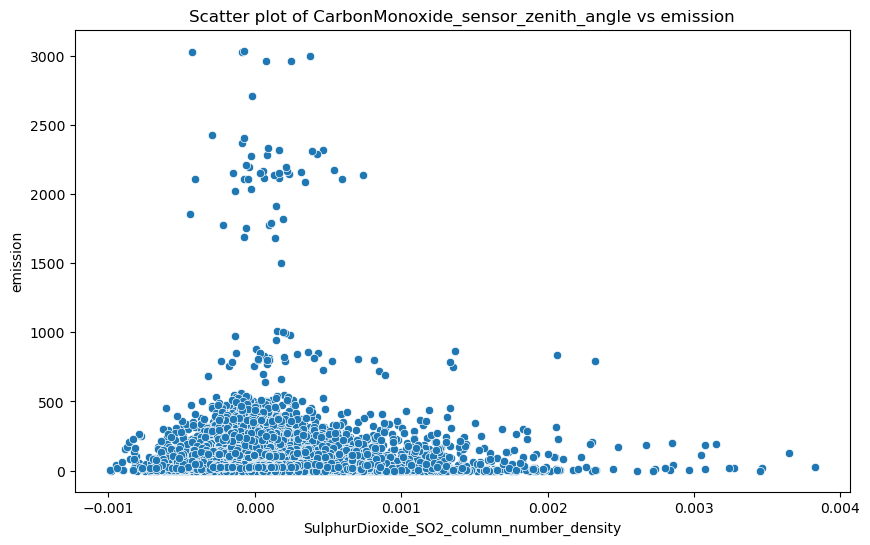
\includegraphics[width=0.8\textwidth]{output1.png}
      \caption{\texttt{SulphurDioxide\_SO2\_column\_number\_density} 与 \texttt{emission} 的散点图}
\end{figure}

可以看出,这两者之间的相关性非常小,因此我们认为这些气象数据对于预测二氧化碳排放量的影响可以忽略不计。

我们还对其他气象数据进行了类似的分析,得到的结果也是类似的,因此我们决定舍弃这些气象数据。

\subsection{数据预处理}

\subsubsection{空值处理}

\subsubsection{特殊值处理}

\subsubsection{数据归一化}

\subsection{模型选择}

% \subsubsection{线性回归}

\subsubsection{RandomForest(随机森林)}

\subsubsection{CatBoost(类别提升)}

\subsubsection{RadiusNeighbors(半径近邻)}

\subsubsection{KNeighbors(K近邻)}

% \subsubsection{MLPRegressor(多层感知器)}

% \subsubsection{SVR(支持向量回归)}

% \subsubsection{XGBRegressor(XGBoost回归)}

% \subsubsection{LGBMRegressor(LightGBM回归)}

% \subsubsection{AdaBoostRegressor(AdaBoost回归)}

% \subsubsection{GradientBoostingRegressor(梯度提升回归)}

\section{评估}

\section{团队成员分工}

\subsection{吕思翰}

\subsection{来泽远}

\subsection{曹宸瑞}

\section{个人总结与感悟}

\ctexset{bibname=参考文献}
\begin{thebibliography}{100}
\bibitem{ref1}\href{https://www.kaggle.com/code/ambrosm/pss3e20-eda-which-makes-sense}{PSS3E20 EDA which makes sense}
\bibitem{ref2}\href{https://www.kaggle.com/code/kacperrabczewski/rwanda-co2-step-by-step-guide}{Rwanda CO2: Step by step guide}
\end{thebibliography}

\end{document}
